% CHAPTER 3: REQUIREMENTS ANALYSIS
% ======================================================================
{\fontsize{18}{22}\selectfont\textbf{3 Requirements Analysis}}\par

\vspace{3mm}

\subhead{3.1 Banking Industry Context}

The system requirements are derived from banking operations. Banking IT environments share four characteristics that drive the platform's requirements. (i) Large relational databases store client profiles, transaction histories, product catalogs, and compliance records. (ii) Policy and procedure repositories span multiple departments, each document carrying a security classification and subject to frequent regulatory updates. (iii) Administrative workflows such as room booking, calendar coordination, travel planning consume substantial staff hours and remain largely manual. (iv) Security and compliance obligations, including those mandated by the HKMA Supervisory Policy Manual (as discussed in Section 2.6), demand role-based access control, department-scoped data isolation, and auditable escalation processes.

Stakeholder analysis identifies five user groups. Business analysts need to query databases without deep SQL knowledge. Compliance officers need to quickly find relevant regulatory clauses with verifiable references. Administrative staff coordinate meetings and schedules across the organization. Departmental administrators manage team membership, document access rights, and approval workflows in their units. System administrators handle platform configuration, manage user permissions, and allocate resources.

\subhead{3.2 Functional Requirements}

The platform's functional requirements are organized by domain. Table 2 summarizes each requirement with its rationale and priority.

\begin{table}[H]
\centering
\small\singlespacing
\caption{Functional Requirements}
\label{tab:functional-requirements}
\begin{tabularx}{\textwidth}{>{\RaggedRight\arraybackslash}p{0.12\textwidth}>{\RaggedRight\arraybackslash}p{0.24\textwidth}>{\RaggedRight\arraybackslash}p{0.34\textwidth}>{\RaggedRight\arraybackslash}p{0.14\textwidth}}
\toprule
\textbf{ID} & \textbf{Requirement} & \textbf{Description} & \textbf{Priority} \\
\midrule
FR1 & User Authentication \& RBAC & Email-format registration with hashed passwords and stateless JWT authentication. Three roles (Admin, Department Admin, End-User) with fine-grained permissions enforced at the gateway level. & High \\
\midrule
FR2 & Department Management & Hierarchical department structure with six banking units. Department administrators can manage membership and assign clearance levels (Public, Internal, Confidential). & High \\
\midrule
FR3 & Document Management with Security Clearance & Documents stored with department ownership and security level. Access granted only when the user's department and clearance meet the document's requirements. Inaccessible documents trigger a human-in-the-loop escalation pathway. & High \\
\midrule
FR4 & Notification System & Multi-type notifications (chat, access request, SQL audit alert) with a five-state state machine. Unread badge and role-specific views provided on the frontend. & Medium \\
\midrule
FR5 & Code Agent --- NL2SQL & Natural language to SQL translation with security validation before execution. Schema metadata cached to improve generation accuracy. Human-in-the-loop mode supported: generate, review, then execute. & High \\
\midrule
FR6 & RAG Agent --- Policy Q\&A & Natural language questions answered from organizational documents with verifiable source citations. Retrieval filtered by the user's department and clearance level. & Medium \\
\midrule
FR7 & Tool Agent --- Task Automation & Unified natural language interface for meeting room booking, schedule conflict detection, and route planning. Intent recognized automatically and routed to the appropriate handler. & Medium \\
\midrule
FR8 & Admin Resource Management & Role-restricted CRUD endpoints for meeting rooms and schedules. Validation rules enforce required fields, positive capacity, and chronological time ranges. & Medium \\
\bottomrule
\end{tabularx}
\end{table}

\subhead{3.3 Non-Functional Requirements}

NFR1 -- Data Sovereignty. All core data tasks run inside our own Docker setup. These tasks include AI model runs,  finding documents and database work. They all happen in a Docker environment on our own machines. External calls (the DeepSeek LLM endpoint at maas-api.cn-huabei-1.xf-yun.com and the Amap geocoding/routing API at restapi.amap.com) transmit only the minimum required parameters (prompts and coordinates), with no payload logging or retention by third-party providers. All external API keys are stored in environment variables, with development fallback defaults.

NFR2 -- Performance. The system should meet these latency targets: (a) Code Agent SQL generation ≤3 s; (b) Tool Agent meeting-room and schedule queries ≤500 ms; (c) route-planning responses ≤2 s (limited by the Amap API round-trip); (d) WebSocket progress updates ≤200 ms; and (e) initial page load ≤3 s.

NFR3 -- Security. All API traffic must be encrypted with HTTPS/TLS (and WSS for WebSocket connections). User passwords are hashed with BCrypt (strength factor 10). JWT tokens have configurable expiry (default 24 h) and are signed with HMAC-SHA. Method-level authorization is enforced by Spring Security's @PreAuthorize annotations. SQL injection is prevented through the use of PreparedStatement. MyBatis-Plus supports logical deletion. It uses the @TableLogic annotation for this. This works for all entities. It keeps the data for audit purposes.

NFR4 -- Reliability and Availability. The platform is designed to be up 99.5\% of the time during business hours. The system can keep working at a reduced level when some services fail. When the DeepSeek or Amap services cannot be reached, the Tool Agent uses mock data. If the Code Agent's inference server is not available, the system returns error messages. All task failures are logged. They include details like user ID, request payload, and stack trace. This is used for analysis after an incident.

NFR5 -- Maintainability. The architecture follows microservice principles. It keeps different responsibilities separate. Each service provides RESTful APIs. These are documented in Appendix B. A Result<T> wrapper is used for responses. It has code, message, and data. This gives consistent error handling across the whole stack. MyBatis-Plus provides type-safe CRUD operations. It automatically maps underscores to camelCase. It supports logical deletion. It also logs SQL for debugging.

NFR6 -- Deployability. The system is deployed with one Docker Compose command. The MySQL container starts on its own. It uses a file from docker/init/agent\_platform\_backup\_utf8.sql. This file creates all 11 tables with seed data. Service URIs are set through environment variables. Examples are USER\_SERVICE\_URI, TOOL\_SERVICE\_URI, and CODE\_SERVICE\_URI. The default for development is localhost. Health-check probes test if a service is ready. They run before dependent containers start.

\subhead{3.4 Use Case Analysis}

Use case analysis captures how users interact with the multi-agent platform. Figure \ref{fig:tool-agent-usecase} shows the use cases for the Tool Agent module. Three main actors interact with the system. The first group is end users. They have the role ROLE\_USER. They can book meeting rooms, check schedule conflicts and plan routes. The second group is administrators. They have the role ROLE\_ADMIN. They can also manage meeting room and schedule resources. Besides, they can use dedicated admin controllers to do this. There are also two external system actors. One is the DeepSeek LLM. It classifies what the user wants and pulls out parameters from natural language requests. The other is the Amap API. It converts addresses into coordinate and can also calculate routes.

\begin{figure}[H]
\centering
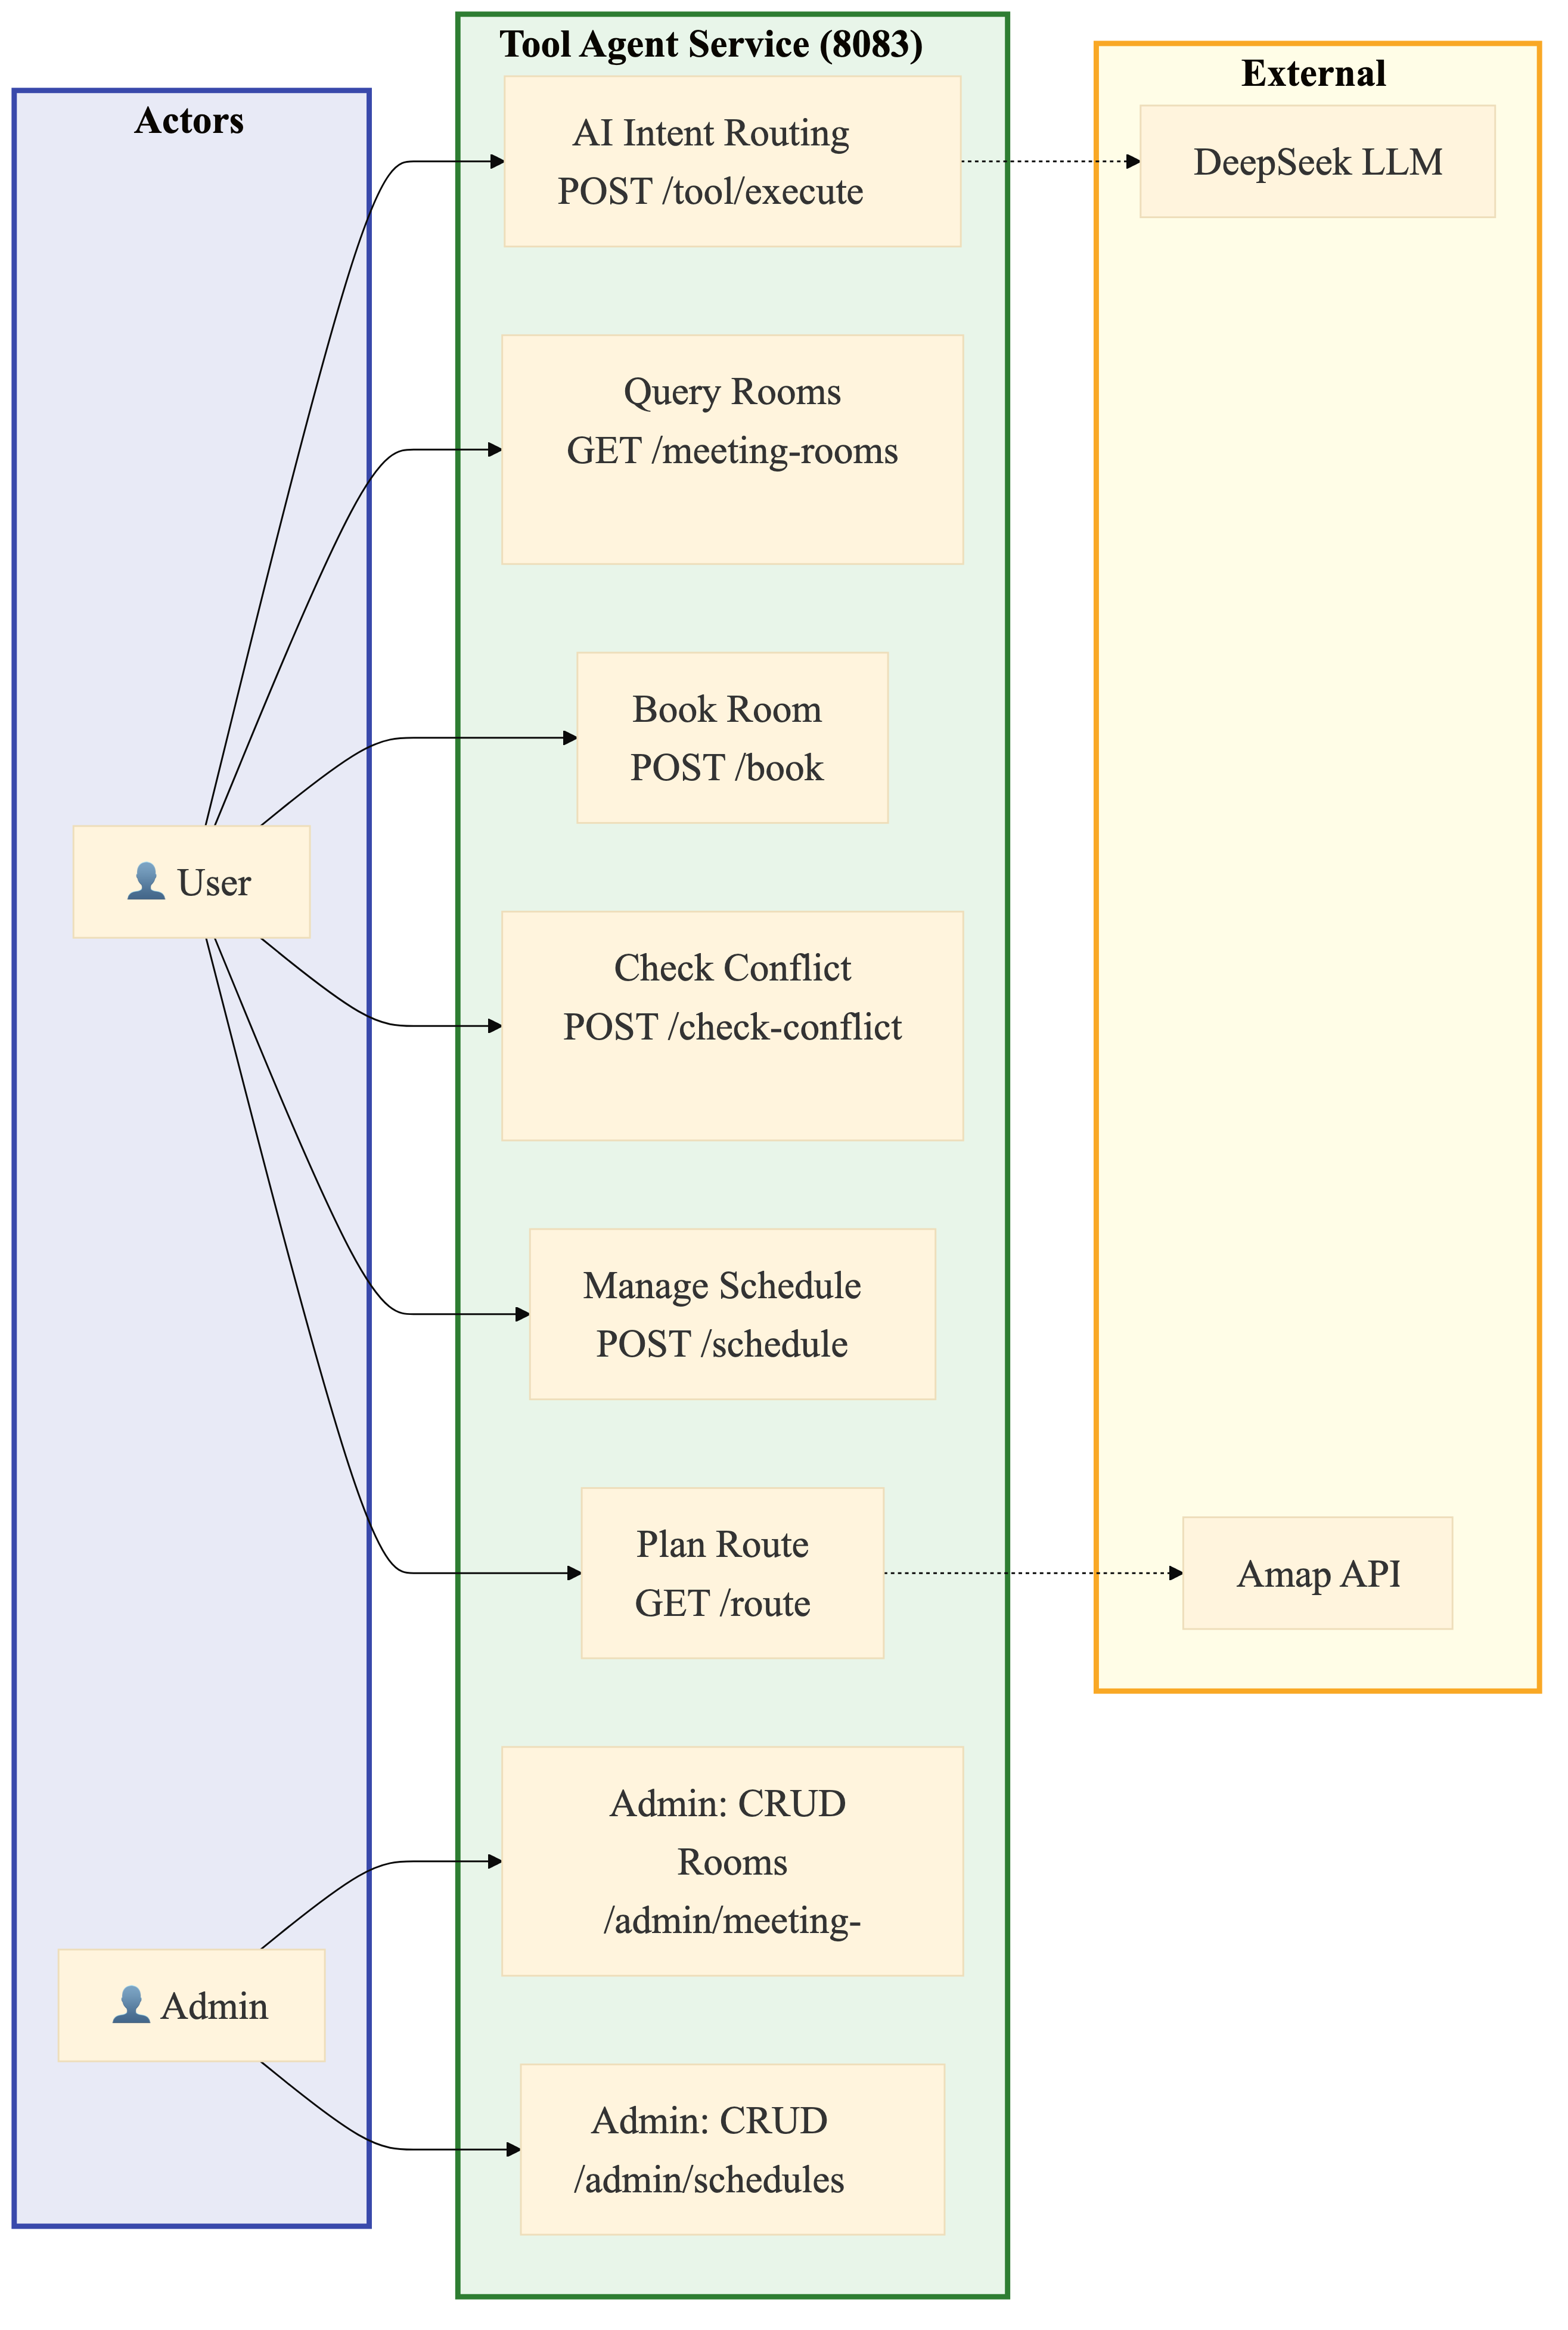
\includegraphics[width=0.92\textwidth]{figures/fig01_tool_agent_usecase.png}
\caption{Tool Agent Use Case Diagram --- Meeting Room, Schedule Conflict, and Route Planning}
\label{fig:tool-agent-usecase}
\end{figure}

There are three agent modules. Their use cases are as following.

UC1 -- Generate SQL from Natural Language (Code Agent). A business analyst types a natural language request. An example is: "Show me all customers who opened accounts in Q1 2026 with balances exceeding HKD 500,000." The CodeAgentController receives the request at the endpoint POST /code/query. It sends the question to the Python LLM inference server on port 8090. The server returns the generated SQL. The five-layer SqlValidationService then checks the SQL. After it passes, the SQL is run through JdbcTemplate with a PreparedStatement. The system returns the result in table form. The result includes column names, row data, and execution time.

UC2 -- Policy Compliance Query (RAG Agent). A compliance officer asks a question. For example: "What are the latest KYC requirements for corporate account opening?" The system encodes the query. It retrieves the top-k most similar document chunks from the Milvus vector store. These chunks are filtered by the user's department and clearance level. The system passes these chunks as context to the LLM. It returns an answer with citations. The citations point to the specific policy documents and sections used.

UC3 -- Meeting Room Booking (Tool Agent). An administrative staff member types a request into the AI Assistant panel. The request is: "Book a meeting room on the 3rd floor for 10 people tomorrow morning at 10 AM." The frontend opens a WebSocket connection. It sends the query. It displays progress. The DeepSeekService classifies the request as MEETING\_QUERY. It extracts the parameters. The parameters are floor 3, capacity 10, and time tomorrow 10:00 AM. The result is sent to the MeetingAgent component. MeetingAgent queries MySQL for rooms that match. It checks the floor and capacity, and then cross-references Redis for time availability. The available options are displayed.

UC4 -- Schedule Conflict Detection (Tool Agent). A user enters a request: "Check if Zhang and Li are free next Tuesday 2-4 PM." The AI identifies the user's intent and then extracts the attendees' names and time range. The ScheduleAgent component calls API and sends the attendee list. The ToolController will check each attendee's schedule. The response shows if conflicts exist, identifies the conflicting users and gives the conflict type with suggested alternatives.

UC5 -- Document Access Escalation (User Center). A Credit Department staff member has clearance Level 1. They try to access a Level-3 confidential risk evaluation document. The method SysDocumentServiceImpl.listDocumentsForUser() checks the access rule. The document's department matches the user's department. But the user's clearance level is 1. This is lower than the document's clearance which is 3. So the document is not accessible. The user can then submit an escalation request, which will create a notification. The notification status starts as Pending and goes to a department administrator for review. The status can be changed to Approved. The approval creates a record that can be audited. Then the user can access the document.

\newpage

% ======================================================================
